
\documentclass[12pt]{article}


\usepackage[T1]{fontenc}
\usepackage[utf8]{inputenc}
\usepackage{amsmath,amssymb}
\usepackage{graphicx}
\usepackage{pgfgantt}
\usepackage[table]{xcolor}
\usepackage{enumitem}

\usepackage{hyperref}


% Blue palette (A1 → A3)
\definecolor{Aone}{HTML}{1F4E79}     % dark blue
\definecolor{Atwo}{HTML}{2E75B6}     % medium blue
\definecolor{Athree}{HTML}{9DC3E6}   % light blue

\definecolor{gridgray}{HTML}{E6E6E6}


\newcounter{task}

\newcommand{\taskitem}[2]{%
  \refstepcounter{task}%
  \item[\textbf{T\thetask}\label{#2}] #1
}
\newenvironment{tasks}{
\begin{enumerate}[leftmargin=1.5cm,labelsep=0.5cm,itemsep=.3em]
}{
\end{enumerate}
}
\usepackage[version=4]{mhchem}

\usepackage[
    top=2cm,
    bottom=2cm,
    left=2cm,
    right=2cm
]{geometry}

\usepackage[
    backend=biber,
    style=authoryear,
    doi=true,
    url=false,
    sorting=nyt,
    maxcitenames=2,
    giveninits=true
]{biblatex}

\addbibresource{isotopes.bib}

\setcounter{subsection}{0}
\renewcommand{\thesubsection}{A\arabic{subsection}}

\title{
    \textbf{A closure study to validate a novel isotope-aware
    Lagrangian cloud-microphysics model\\ against airborne measurements}\\[0.4em]
    \large Próba zgodności z pomiarami lotniczymi nowego lagranżowskiego modelu
    mikrofizyki chmur obejmującego zjawiska izotopowe
}

%\author{
%Agnieszka Żaba\\
%AGH University of Krakow
%}
\date{}


\begin{document}
\maketitle
\section{Scientific goal of the project}
Water stable isotopologues are natural tracers of the global hydrological cycle.
Variations in isotopic composition arise from isotope fractionation accompanying
phase transitions and transport processes in the atmosphere.
Consequently, the isotopic composition of atmospheric water preserves information
about the thermodynamic and microphysical history of air parcels, clouds,
and precipitation.

In atmospheric sciences, the water isotopologues most commonly studied are \ce{HDO},
\ce{H2{}^18O}, and \ce{H2{}^17O}.
Their relative abundances differ from that of the dominant isotopologue \ce{H2{}^16O},
leading to measurable fractionation during evaporation, condensation, and mixing processes.
Recent advances in cavity-enhanced laser spectroscopy have enabled continuous,
high-precision measurements of multiple water isotopologues in atmospheric water vapour,
including triple oxygen isotopes, especially \ce{^17O}.
Measurements of the isotopic composition of water vapour below cloud base will provide input
to a particle-resolved cloud model.
The simulated cloud state will subsequently be evaluated against observational data.
The overall objective is to reconstruct cloud isotopic conditions using numerical simulations.

A central question is whether isotopic measurements provide sufficient information
to constrain cloud microphysical processes and achieve isotopic closure within
a prognostic particle-based framework.
More broadly, it remains unknown whether isotopic closure can be achieved with current
measurement capabilities and advances in particle-based cloud modelling.
If so, an equally important question is what constitutes the minimal mathematical model,
numerical implementation, and observational framework required to achieve it.

In this context, fluctuations in supersaturation play a key role in governing
condensation and evaporation rates at the particle level, thereby influencing
both cloud microphysics and isotopic partitioning.
Recent work has shown that
haze–cloud interactions can be strongly modulated
by supersaturation variability
\parencite{2026_FahandezhSadi_EtAl}.

The project addresses the following research questions:
\begin{enumerate}
    \item[\textbf{Q1}] Can isotopic closure be achieved in a particle-based
        cloud model using currently available isotopic observations?
    \item[\textbf{Q2}] Which cloud microphysical processes leave
        identifiable signatures in the isotopic composition
        of atmospheric water?
    \item[\textbf{Q3}] To what extent do isotopic measurements constrain
        key cloud properties such as supersaturation variability,
        phase partitioning, and mixing?
    \item[\textbf{Q4}] What is the minimal physical and numerical
        framework required to achieve isotopic closure
        while maintaining predictive skill?
\end{enumerate}


\section{Significance of the project}
Cloud microphysical processes remain one of the largest sources of
uncertainty in weather prediction and climate projections \parencite{IPCC_2023}.
Processes such as condensation, evaporation, entrainment,
and phase transitions between liquid water and ice strongly
influence cloud lifetime, precipitation formation,
and radiative properties.
Yet many of these processes cannot
be directly observed and therefore remain poorly constrained
in atmospheric models \parencite{2013_Grabowski_Wang}.

Stable water isotopologues provide a unique observational tracer 
of cloud evolution.
During phase transitions, isotopic fractionation modifies
the relative abundance of isotopologues in vapour, liquid water, and ice \parencite{2017_Lamb_EtAl}.
Consequently, isotopic composition contains information about 
the thermodynamic and microphysical history of air masses and
clouds \parencite{2013_Bolot_EtAl}.

Theoretical descriptions of equilibrium and kinetic isotope
fractionation are well established,
and stable water isotopologues are routinely represented
in global and regional atmospheric models \parencite{2016_Galewsky_EtAl}.
These isotope-enabled models have significantly improved
understanding of large-scale moisture transport and
the atmospheric hydrological cycle \parencite{2020_Risi_EtAl}.
However, most %of? many? 
existing approaches rely on Eulerian formulations
and bulk cloud parameterisations,
limiting their ability to resolve the particle-scale processes
responsible for generating isotopic signatures.

At the same time, particle-based cloud models have emerged 
as a state-of-the-art framework for studying cloud microphysics \parencite{2009_Shima_EtAl}.
By explicitly representing aerosol particles, cloud droplets,
and ice particles, these models provide detailed descriptions of condensation,
evaporation, freezing, and other microphysical processes.

Despite these advances, isotopic composition has rarely been 
considered within particle-based cloud modelling,
and its potential as a constraint on cloud evolution remains
largely unexplored.
A~fundamental unresolved question is whether isotopic observations
contain sufficient information to constrain cloud microphysical
processes and achieve isotopic closure.
Analogously to cloud condensation nuclei closure studies,
isotopic closure can be understood as the ability to consistently explain observed
isotopic composition using a physically based description of cloud evolution \parencite{2021_Knopf_EtAla}.
While isotopic measurements are increasingly available and
process-resolving cloud models are becoming increasingly sophisticated,
no systematic framework currently exists for assessing isotopic
closure in cloud systems.

The proposed project addresses this gap by investigating isotopic
closure using process-resolving cloud simulations and isotopic observations
from in-cloud measurements and laboratory experiments.
The project is pioneering because it introduces isotopic closure
as a research objective in cloud physics and establishes
a link between isotope-enabled observations and modern cloud microphysics.
The results will provide insight into the information content
of isotopic measurements, improve understanding of isotopic signatures
generated by cloud processes, and contribute to the development
of new observational constraints for atmospheric modelling.

\section{Research Concept and Work Plan}
The project is divided into three areas: development of a physically
consistent theoretical description of isotopic fractionation (\ref{A1}),
its implementation in a particle-based cloud microphysics framework (\ref{A2}),
and evaluation against observational and laboratory data (\ref{A3}).
Feedback between these components ensures continuous refinement
of both model formulation and interpretation of isotopic signals.

\subsection{Theory: isotopic cloud microphysics}\label{A1}
This research area focuses on developing a unified theoretical framework for
isotopic fractionation in liquid-vapour-ice systems.
The objective is to formulate governing equations that
describe isotope-specific mass transfer in
cloud environments, including both equilibrium and kinetic processes.
The~analysis will include:
(i) derivation of isotopic mass balance equations for vapour, liquid, and ice
phases,
(ii) identification of limiting regimes such as equilibrium fractionation and
Rayleigh-type distillation,
and (iii) formulation of dimensionless control parameters, including the Bolin
Number introduced in preliminary studies.

A key objective is to identify the minimal set of physically
essential processes that govern isotopic signatures in clouds.
This includes condensation, evaporation, deposition, sublimation,
and freezing, expressed in a~form consistent with particle-based modelling.
The outcome of~\ref{A1} is a~closed and consistent theoretical description
of isotopic cloud microphysics suitable for numerical implementation.

In addition to model validation, the proposed framework includes
a~systematic analysis of numerical model errors,
sensitivity to key physical parameters,
and uncertainty propagation within the isotopic closure framework. 
This encompasses both local sensitivity analysis of governing 
equations and global sensitivity studies based on numerical experiments.

Uncertainty propagation will be quantified through ensemble simulations,
allowing assessment of how uncertainties in microphysical parameters,
initial conditions, and isotopic boundary conditions influence
the simulated isotopic composition.
Particular attention will be given to distinguishing
structural model uncertainty from observational uncertainty.

\subsection{Numerics: particle-based implementation and simulation framework}\label{A2}
This research area focuses on implementing the theoretical framework within a
particle-based cloud microphysics model based on the Super-Droplet Method (SDM)
in the PySDM environment.
The model will be extended to include prognostic tracking of multiple water
isotopologues in vapour, liquid, and ice phases at the level of individual
computational particles.
This enables explicit representation of isotopic
fractionation associated with phase transitions, diffusive exchange and collisions
simultaneously for all isotopologues considered in analysis.
The implementation will follow reproducible scientific software practices,
including modular design, automated testing, and continuous integration.

Physical consistency will be ensured through conservation checks and validation
against analytical limiting solutions.
Numerical experiments will be performed in idealised configurations,
including box, parcel, and column models.
These simulations will isolate the response of
isotopic composition to key environmental and microphysical controls, such as
supersaturation, temperature, droplet size distribution, and ice fraction.

The outcome of~\ref{A2} is a~validated isotope-enabled particle-based modelling
framework capable of simulating cloud evolution with explicit isotopic
tracking.

\subsection{Data: observational and experimental validation}\label{A3}
This research area is dedicated to assessing model predictions through
comparison with observational data.
This research area focuses on evaluating model predictions against data.
The model will be tested using isotopic measurements from aircraft campaigns,
including the CAESAR dataset, as well as laboratory experiments
performed in collaboration with NSF NCAR (Elise Rosky).
Together, these datasets offer complementary constraints spanning vapour,
cloud water, ice, and precipitation phases.

The laboratory component is currently in a~preliminary stage,
and its design will evolve in parallel with the development
of the modelling framework.
This co-development approach highlights the potential and scientific
importance of the proposed project,
as it enables direct feedback between numerical modelling
and experimental design.
It also ensures consistency between observational capabilities,
experimental constraints, and the evolving requirements of the analysis,
while supporting close interdisciplinary collaboration.

The analysis will focus on three aspects:
(i) agreement between simulated and observed isotopic composition,
(ii) sensitivity of isotopic signals to cloud microphysical processes, and
(iii) ability of isotopic measurements to constrain cloud evolution and assess
closure.
The outcome of A3 is an empirical evaluation of isotopic closure and a
quantification of the information content of isotopic observations in
mixed-phase cloud systems.



\subsection*{Integration of A1--A3}
The three research areas are strongly coupled.
\ref{A1} defines the physical
description of isotopic processes,
\ref{A2} translates this description into a
numerical particle-based framework,
and~\ref{A3} provides observational constraints
and validation.
This integrated structure enables a~systematic investigation of isotopic
closure, ensuring consistency between theory, numerical representation, and
observational evidence.



\section*{Preliminary Results} 
The proposed research builds on results obtained within a~previous NCN project
in which the PI contributed to the development of isotope-enabled particle-based
cloud modelling.
These preliminary studies provide a~proof-of-concept for the
feasibility of prognostic isotopic tracking in Lagrangian cloud microphysics
and form a direct foundation for the present proposal.

\subsection*{\ref{A1} -- Theory: Dimensionless formulation of isotopic evolution}
A~dimensionless framework for describing isotopic evolution in particle-based
cloud models was introduced through the concept of the Bolin number.
The formulation builds on the original work of \textcite{1958_Bolin},
originally developed for tritium transport in atmospheric water.

The Bolin number expresses the relative strength of
diffusive and phase-change-driven isotopic exchange between isotopologues.
It is defined as:
$\textbf{Bo} = \frac{\tau_\text{heavy}}{\tau_\text{light}} \approx \frac{\tau_\text{heavy}}{\tau_\text{total}}$,
 where $\tau = \left(\frac{1}{m} \frac{dm}{dt}\right)^{-1}$
 represents the characteristic equilibration timescale of a~given water isotopologue.
By defining this number explicitly, the evolution of a~heavy isotopologue can be
 inferred from the dynamics of the mass of the light isotopologue (or approximately
 of the droplet total mass).
The use of the Bolin number simplifies model formulation by capturing
 the efficiency of isotopic fractionation in a~single dimensionless value.
It incorporates quantities such as the equilibrium fractionation factor $\left(\alpha_\text{eq}\right)$;
heat conduction and mass diffusion (including ventilation); and environmental conditions such as temperature
 and saturation ratio.
This reduction leads to a~compact, physically interpretable representation of
isotopic evolution, which captures both equilibrium and kinetic fractionation
regimes within a~unified framework.

\subsection*{\ref{A2} -- numerics: Particle-based implementation and numerical validation}
Isotopic evolution of water vapour and cloud droplets for one heavy isotopologue has been implemented within
the Super-Droplet Method (SDM) framework \parencite{2009_Shima_EtAl}.
The implementation was developed within the PySDM environment \parencite{2022_Bartman_EtAl, 2023_DeJong_EtAl}
and extended to include prognostic isotopic composition of individual computational particles.

The implementation of the Bolin number was validated against equilibrium
isotopic fractionation 
curves for water vapour and liquid phases
\parencite{1994_Gedzelman_Arnold}.
A~schematic interpretation of isotopic equilibration regimes in relation to the
Bolin number is shown in Fig.~\ref{fig:bolin}.

\begin{figure}[htbp]
    \centering
    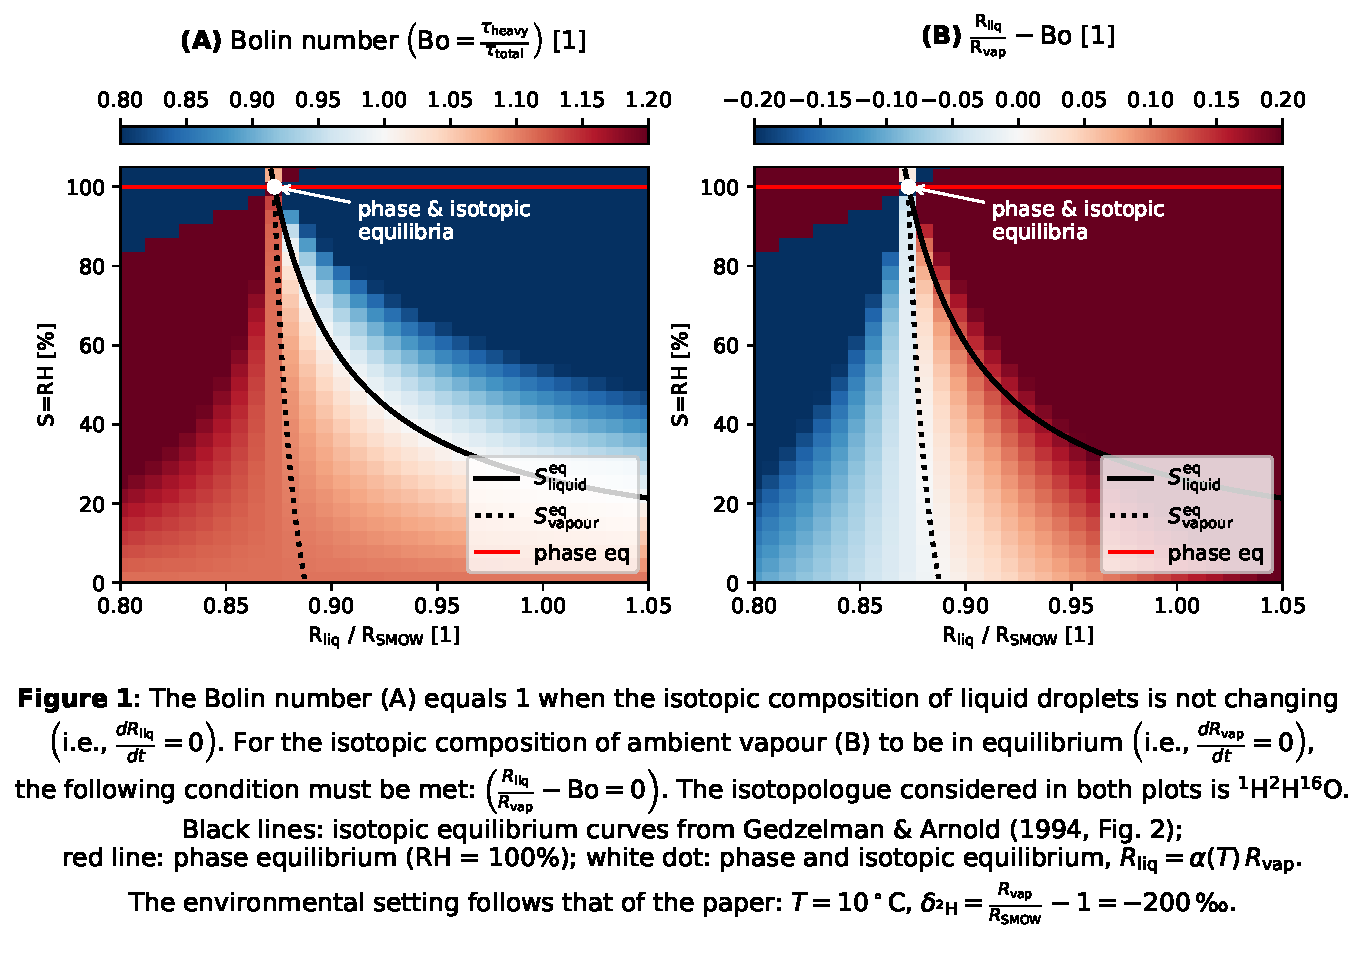
\includegraphics[width=.7\textwidth]{Bo} 
    \caption{Conditions for isotopic steady state in liquid droplets (A)
        and ambient vapour (B).
        Panel A~shows the locus where the isotopic composition
        of liquid water remains constant ($\left(dR_{\mathrm{liq}}/dt=0\right)$),
        corresponding to ($\mathrm{Bo}=1$).
        Panel B shows the locus where the isotopic composition of vapour
        remains constant ($\left(dR_{\mathrm{vap}}/dt=0\right)$),
        corresponding to ($R_{\mathrm{liq}}/R_{\mathrm{vap}}-\mathrm{Bo}=0$).
        The figure illustrates the theoretical equilibrium relationships governing
        isotopic exchange between liquid and vapour phases. 
        The isotopologue considered is ($^{1}\mathrm{H}^{2}\mathrm{H}^{16}\mathrm{O}$).
        Black lines indicate isotopic equilibrium curves, the red line phase equilibrium (RH = 100$\%$),
        and the white dot simultaneous phase and isotopic equilibrium.
}
    \label{fig:bolin}
\end{figure}
The developed concept has been accepted for presentation at the 17th Conference
on Cloud Physics (AMS Madison Summit 2026), where it will be presented to the
atmospheric science community as a~novel particle-based formulation of isotopic
cloud microphysics.


\section{Project Tasks, Milestones and Schedule}
The task structure follows the three research areas defined in the project concept (\ref{A1}, \ref{A2}, \ref{A3}),
ensuring consistency between theoretical development,
numerical implementation, and data-driven evaluation.
This structure supports iterative feedback between model formulation
and physical interpretation of isotopic signals.

The research plan is formulated according to
the SMART principle (specific, measurable, achievable, relevant, and time-bound).
Each work package is decomposed into specific tasks.

\subsection*{Tasks}
\subsection{Theory: Isotopic Cloud Microphysics}

\begin{tasks}
    \taskitem
    {Isotope-specific governing equations and mixed-phase Bolin number.
    Develop a unified mathematical framework describing isotopic mass transfer
    among vapour, liquid, and ice phases, including equilibrium and kinetic
    fractionation and extension of the Bolin number.}
    {task:T1}
    \\\textbf{Deliverable}: Mathematical formulation of mixed-phase isotope cloud microphysics.

    \taskitem
    {Reduced-order models. Identify limiting regimes including equilibrium,
    Rayleigh distillation, and diffusion-limited growth.}
    {task:T2}
    \\\textbf{Deliverable}: Reduced models for closure analysis.

    \taskitem
    {Sensitivity and uncertainty analysis of isotopic evolution.}
    {task:T3}
    \\\textbf{Deliverable}: Sensitivity maps and uncertainty framework.
\end{tasks}


\subsection{Numerical Framework: Particle-Based Implementation}

\begin{tasks}
    \taskitem
    {Box, Parcel, and One-Column isotope-enabled simulations with validation.}
    {task:T4}
    \\\textbf{Deliverable}: Jupyter notebook collection.
    
    \taskitem
    {Ice-phase isotope microphysics and multi-isotopologue (\ce{HDO}, \ce{H2^{18}O}, \ce{H2^{17}O}).}
    {task:T5}
    \\\textbf{Deliverable}: Ice-phase module with unit tests.
    
    \taskitem
    {Minimal isotope-enabled cloud model for closure studies.}
    {task:T6}
    \\\textbf{Deliverable}: Open-source model with documentation.
\end{tasks}

\subsection{Validation and Closure Assessment}

\begin{tasks}
    \taskitem
    {Preparation of observational and laboratory datasets with uncertainty characterization.}
    {task:T7}
    \\\textbf{Deliverable}: Data-processing pipeline and emulator.
    
    \taskitem
    {Data--model comparison using quantitative diagnostics.}
    {task:T8}
    \\\textbf{Deliverable}: Model performance metrics.
    
    \taskitem
    {Assessment of isotopic closure and required physical constraints.}
    {task:T9}
    \\\textbf{Deliverable}: Closure framework (Q1–Q4).
\end{tasks}




\subsection*{Milestones}
The project includes four measurable milestones:

\begin{itemize}
\item[\textbf{M1}]\label{M1} Completion of the theoretical framework for isotope-enabled cloud microphysics, including governing equations and analysis of limiting regimes.
\item[\textbf{M2}]\label{M2} Implementation and validation of particle-based isotope-enabled models, including ice-phase processes and multi-isotopologue representation.
\item[\textbf{M3}]\label{M3} Integration of observational and laboratory datasets with the modelling framework and initiation of systematic model evaluation.
\item[\textbf{M4}]\label{M4} Completion of isotopic closure assessment, including sensitivity and uncertainty analysis and identification of minimal modelling requirements.
\end{itemize}

\subsection*{Schedule}
Tasks are distributed over a 24-month period according 
to their logical and computational dependencies.
Early stages focus on theoretical development (A1),
followed by numerical implementation (A2). 
Data integration and validation (A3) are initiated
once core model components are operational,
enabling iterative refinement through feedback
between modelling and observational constraints.

The temporal allocation of tasks and milestones
is presented in the Gantt chart (\ref{fig:gantt}).

\begin{figure}[t]
\centering
\footnotesize

\begin{ganttchart}[
    hgrid,
    vgrid,
    hgrid style/.style={draw=gridgray, line width=0.3pt},
    vgrid style/.style={draw=gridgray, line width=0.3pt},
    x unit=0.55cm,
    y unit chart=0.55cm,
    bar height=0.7,
    group height=0.8,
    milestone height=0.7,
    progress label text={},
]{1}{24}
\ganttset{
group/.style={
    draw=Aone,
    fill=Aone!20,
    line width=0.6pt
}
}
\gantttitle{Project Duration (Months)}{24} \\
\gantttitlelist{1,...,24}{1} \\

%----------------------------------------------------
% A1 THEORY
%----------------------------------------------------
\ganttset{
bar/.style={
    fill=Aone,
    draw=Aone,
    line width=0.4pt
}
}

\ganttgroup{\ref{A1} Theory}{1}{12} \\

\ganttbar{Task \ref{task:T1}}{1}{6} \\
\ganttbar{Task \ref{task:T2}}{5}{10} \\
\ganttbar{Task \ref{task:T3}}{8}{14} \\

\ganttmilestone{\ref{M1} Theory framework}{6} \\

%----------------------------------------------------
% A2 NUMERICS
%----------------------------------------------------
\ganttset{
bar/.style={
    fill=Atwo,
    draw=Atwo,
    line width=0.4pt
}
}

\ganttgroup{\ref{A2} Numerics}{3}{20} \\

\ganttbar{Task \ref{task:T4}}{3}{10} \\
\ganttbar{Task \ref{task:T5}}{8}{15} \\
\ganttbar{Task \ref{task:T6}}{12}{20} \\

\ganttmilestone{\ref{M2} Numerical framework}{12} \\

%----------------------------------------------------
% A3 VALIDATION
%----------------------------------------------------
\ganttset{
bar/.style={
    fill=Athree,
    draw=Athree,
    line width=0.4pt
}
}

\ganttgroup{\ref{A3} Data}{8}{24} \\

\ganttbar{Task \ref{task:T7}}{8}{13} \\
\ganttbar{Task \ref{task:T8}}{12}{20} \\
\ganttbar{Task \ref{task:T9}}{16}{24} \\

\ganttmilestone{\ref{M3} Data integration}{18} \\
\ganttmilestone{\ref{M4} Closure assessment}{24}

\end{ganttchart}

\caption{
Project timeline structured into three work packages:
\ref{A1} theoretical development, \ref{A2} numerical implementation,
and \ref{A3} validation and closure assessment.
}
\label{fig:gantt}
\end{figure}


\subsection*{Result dissemination}
Project results will be disseminated through peer-reviewed publications,
conference presentations, research visits, and open-source software releases.
Results will be submitted to international journals relevant to atmospheric
modelling and isotope hydrology, including \emph{Tellus B: Chemical and Physical
Meteorology}, \emph{Atmospheric Chemistry and Physics},
\emph{Journal of Advances in Modeling Earth Systems}, and
\emph{Geoscientific Model Development}.
Interim and final results will be presented as talks and posters at
international conferences, including the European Geosciences Union General
Assembly and the International Conference on Clouds and Precipitation.

The project includes a~research visit to the United States, a~visit of an
international collaborator to AGH University, and participation of the MSc
student in an international summer school.
All software developed within the project will be released as open source via
GitHub, accompanied by documentation and reproducible Jupyter notebooks
demonstrating the proposed methods and numerical experiments.
Data-processing
workflows required to reproduce published results will be made publicly
available.



\subsection*{Expected outcome of project execution}
The expected result is a~validated, process-resolved framework for isotopic cloud microphysics
capable of testing the concept of isotopic closure in mixed-phase clouds.
The project will provide both a~computational tool and a~set of physically constrained
benchmarks for future isotope-enabled cloud modelling studies.


\section*{Research methodology}
Underlying scientific methodology, methods, techniques and research tools,
methods of results analysis, and equipment used in the research are based 
on a~combination of physically based modelling, particle-based numerical simulation,
and systematic data-model comparison.

\subsection*{PySDM: Super-Droplet Method and modelling framework}
The numerical core of the model is the Super-Droplet Method (SDM),
a~particle-based Lagrangian framework for cloud microphysics.
In SDM, clouds are represented by computational particles (\emph{super-droplets}),
where each super-droplet represents a~multiplicity of identical real aerosol,
cloud droplet, or ice particles.
This formulation enables explicit representation of stochastic
microphysical interactions while maintaining computational efficiency
at cloud-resolving scales.
SDM couples Lagrangian particle dynamics with Eulerian 
fields describing thermodynamic variables such as temperature,
pressure, and water vapour.
This hybrid structure allows consistent simulation of
cloud–environment interactions.

The method provides explicit treatment of key microphysical processes,
including condensation and evaporation, diffusional growth,
collision–coalescence, as well as ice-phase processes such as deposition,
sublimation, freezing, and melting, without relying on bulk parameterisations.

The model is implemented within the open-source
PySDM framework \parencite{2022_Bartman_EtAl, 2023_DeJong_EtAl}.
PySDM provides a modular environment for particle-based cloud modelling
that includes numerical solvers, a set of microphysical process 
implementations, and diagnostic and analysis tools. 

In this project, PySDM is extended to include prognostic tracking
of multiple water isotopologues in vapour, liquid, and ice phases,
fully coupled to the SDM microphysical framework.
This extension preserves the original particle-based structure
while augmenting each super-droplet with isotopic composition 
as an additional prognostic variable.

\subsection*{Jupyter notebook–based simulation and analysis environment}
A central component of the project is the use of Jupyter notebooks
as the primary interface for model development, numerical experiments,
and data analysis.
Each notebook constitutes a fully self-contained and executable
research workflow, including (i) model configuration and initialization,
(ii) simulation execution,
(iii) post-processing and diagnostics, and 
(iv) visualisation of results.
This design ensures that every numerical experiment is fully reproducible
and can be independently executed without additional external
scripts or hidden dependencies.

Notebooks function simultaneously as: (i) an executable research workflow; (ii) a documentation format;
(iii) and a reproducible dissemination layer for scientific results.
Within this project, notebooks are integrated with version control
and continuous integration (CI) pipelines. 
This ensures that all simulations remain reproducible
over time and that changes in the codebase automatically trigger 
validation of numerical correctness.

\subsection*{Reproducibility, software engineering, and research workflow}
The project follows established reproducible research practices.
All components of the modelling system, including PySDM extensions,
simulation configurations, and analysis notebooks,
are managed in version-controlled repositories and continuously
validated through automated CI pipelines.
The CI system performs:
(i) unit tests verifying physical consistency (e.g. mass conservation and isotopic bounds),
(ii) regression tests ensuring numerical stability across updates,
(iii) and benchmark tests against analytical or well-established reference solutions.
This workflow ensures that model development remains transparent, 
scientifically traceable, and computationally robust.

\subsection*{Educational and training component}
The Jupyter-based workflow plays a key role in the training component
of the project.
The MSc/Erasmus+/PhD student involved in the project will
contribute directly to the development of simulation notebooks, including
simplified educational model configurations,
reproducible experiment templates for key processes,
and interactive visualisation and analysis tools.

This approach lowers the entry barrier to particle-based
cloud microphysics and provides hands-on training in modern
scientific computing, including numerical modelling,
uncertainty quantification, and reproducible research practices.
As a result, the project integrates scientific development
with structured training in computational atmospheric physics.

\section*{Composition and qualifications of the research team}
The research team consists of the Principal Investigator (PI),
a scientific mentor, and one student, 
forming a compact group focused on particle-based cloud microphysics
and isotope-enabled modelling.
\\

\noindent\textbf{Principal Investigator}
The Principal Investigator is a PhD student in the physical
sciences with a background in mathematics and numerical modelling. 
The PI has experience in scientific computing and Python-based development,
with a focus on particle-based atmospheric simulation frameworks.
The PI is the main developer of the isotope-enabled cloud microphysics
framework presented in this proposal, integrating theoretical 
formulations, numerical implementation, and data analysis within
a unified modelling environment.
Previous work includes isotope-enabled cloud modelling 
and international collaboration at 
the National Center for Atmospheric Research (NCAR), 
including work with Dr. Elise Rosky on mixed-phase cloud isotopic processes.
Results was by ER at 
the European Geosciences Union (EGU) General Assembly \parencite{2025_Rosky_MixedPhaseIsotopes}.
\\

\noindent\textbf{Scientific mentor}
The scientific mentor is Dr. Sylwester Arabas,
co-developer of the PySDM particle-based cloud microphysics 
framework and an expert in Lagrangian cloud modelling and 
scientific computing.
The mentor contributes to the development of open-source
atmospheric modelling tools and ensures the physical and numerical 
robustness of the SDM-based framework.
\\

\noindent\textbf{Student contribution}
The student (MSc/Erasmus+/PhD level) will support development
of a~minimal computational environment for isotope-enabled cloud simulations.
The implementation will be in Python (optionally Julia) and will 
serve as a reusable and accessible framework for research and training
in cloud microphysics.
\\

\noindent\textbf{Environmental Physics group background}
The PI and scientific mentor are affiliated with the
Environmental Physics group, which conducts research on atmospheric
isotope systematics and tracer-based hydrological processes.
The group has experience in the measurement, analysis,
and interpretation of stable water isotopes in environmental
and atmospheric applications, including diffusion and phase-change
fractionation processes \parencite{2022_Pierchala_EtAl}.
This background supports the integration of isotope observations
with particle-based cloud modelling and provides methodological 
continuity between observational and numerical approaches.

\appendix

\clearpage
\printbibliography
\end{document}